% -----------------------------------------------
% Template for ISMIR Papers
% 2020 version, based on previous ISMIR templates

% Requirements :
% * 6+n page length maximum
% * 4MB maximum file size
% * Copyright note must appear in the bottom left corner of first page
% * Clearer statement about citing own work in anonymized submission
% (see conference website for additional details)
% -----------------------------------------------

\documentclass{article}
\usepackage[T1]{fontenc} % add special characters (e.g., umlaute)
\usepackage[utf8]{inputenc} % set utf-8 as default input encoding
\usepackage{ismir,amsmath,amssymb,cite,url}
\usepackage{graphicx}
\usepackage{color}

% Optional: To use hyperref, uncomment the following.
\usepackage[bookmarks=false,hidelinks]{hyperref}
% Mind the bookmarks=false option; bookmarks are incompatible with ismir.sty.

\usepackage{lineno}
%\linenumbers

% Custom commands:
% ~~~~~~~~~~~~~~~~
\newcommand{\TODO}[1]{{\Large \color{red} TODO #1}}

\DeclareMathOperator*{\argmax}{argmax}
\DeclareMathOperator*{\argmin}{argmin}

\DeclareMathOperator{\RR}{\mathbb{R}}
\DeclareMathOperator{\EE}{\mathbb{E}}
\DeclareMathOperator{\tr}{\text{tr}}
\DeclareMathOperator{\sg}{\text{sg}}
\DeclareMathOperator{\Softmax}{\text{Softmax}}
\DeclareMathOperator{\Sim}{\text{sim}}

% Title.
% ------
\title{Spectrogram Inpainting: Discrete latent representations for lightweight Interactive Audio Effects}

% Note: Please do NOT use \thanks or a \footnote in any of the author markup

% Single address
% To use with only one author or several with the same address
% ---------------
%\oneauthor
% {Names should be omitted for double-blind reviewing}
% {Affiliations should be omitted for double-blind reviewing}

% Two addresses
% --------------
%\twoauthors
%  {First author} {School \\ Department}
%  {Second author} {Company \\ Address}

%% To make customize author list in Creative Common license, uncomment and customize the next line
%  \def\authorname{First Author, Second Author}


% Three addresses
% --------------
% \fourauthors
%   {Paul Chable} {IRCAM, Paris, France \\ {\tt chable@ircam.fr}}
%   {Jeffery Durand} {IRCAM, Paris, France \\ {\tt durand@ircam.fr}}
%   {Yvan Giro} {IRCAM, Paris, France \\ {\tt giro@ircam.fr}}
%   {Alain Riou} {IRCAM, Paris, France \\ {\tt riou@ircam.fr}}

%% To make customize author list in Creative Common license, uncomment and customize the next line
%  \def\authorname{First Author, Second Author, Third Author}

% Four or more addresses
% OR alternative format for large number of co-authors
% ------------
\multauthor
{Paul Chable \hspace{1cm} Jeffery Durand \hspace{1cm} Yvan Giro \hspace{1cm} Alain Riou} { \\
IRCAM, Paris, France\\
{\tt\small lastname@ircam.fr}
}
%\def\authorname{First author, Second author, Third author, Fourth author, Fifth author, Sixth author}


\sloppy % please retain sloppy command for improved formatting

\begin{document}

%
\maketitle
%
\begin{abstract}% à relire
Learning lightweight representations of audio samples is a key challenge of real-time music generation.
The main purpose of this project was to implement Vector Quantized-Variational Autoencoders (VQ-VAE) to learn discrete representations of audio effects and then to generate new ones using a naive Bayes classifier on the learned codemaps.
In order to evaluate the quality of our models, we performed several experiments on images and spectrograms.
We also created a real-time CO$_2$ tracker in order to track the energy consumption induced by our experiments while training.

This document presents the different models we used during this project and details the results of our experiments on MNIST and NSynth datasets.
The whole implementation of the project is available on GitHub\footnote{\href{https://github.com/aRI0U/spectrogram-inpainting}{\tt github.com/aRI0U/spectrogram-inpainting}}.
\end{abstract}
%
\section{Introduction}\label{sec:introduction}

Research in computer music aims at providing musicians with innovative tools that make use of recent findings and developments in fields such as machine learning. Indeed, generative models represent a very active subject of research, as new models are regularly proposed and refined. Notable examples are the Generative adversarial network-based GANSynth~\cite{GANSynth}, or the use of WaveNet-style autoencoders~\cite{NSynth, WavenetSpeech}, that both propose high-fidelity audio synthesis. These applications allow to create interesting sounds without any input, but generative models can also be exploited in other contexts, such as the alteration of an existing sound.

This project aims at providing a simple digital audio effect that transforms an audio signal locally in its time-frequency representation in real-time, by regenerating parts of it. This is the principle of \textbf{spectrogram inpainting}. Regenerating portions of a spectrogram implies developping a model that is able to learn a probability distribution of each point of the spectogram, based on their neighbours. This problem is approached with a recently proposed generative model, the Vector Quantized - Variational AutoEncoder (VQ-VAE), derived from the usual Variational AutoEncoder. Examples in the litterature of musical applications of the VQ-VAE include Jukebox~\cite{Jukebox}, a model that generates music with singing in the raw audio domain (by contrast with the use of symbolic information such as MIDI). The idea motivating the use of the VQ-VAE is to compress spectrograms into an extremely compact grid that is then quantized into a codemap, made out of a selected amount of codewords. Finally, the decoder reconstructs a spectrogram. Inpainting is performed through Bayesian inference.\\

This document is organized in several sections~: in section~\ref{sec:background}, the general principles behind the VQ-VAE are presented. In section~\ref{sec:MNIST}, the MNIST dataset is introduced and is used to test the proposed model. Section~\ref{sec:NSynth} presents the NSynth dataset and the considerations that come with training a model on audio files. Throughout the project, the question of the environmental cost of machine learning is raised. The carbon footprint of our model's training is estimated and discussed in Section~\ref{sec:energy}. Finally, the produced audio effects are presented in Section~\ref{sec:experiments}.

\section{Background: VQ-VAE}\label{sec:background}

A Variational Autoencoder (VAE) consists of an encoder network, a prior distribution $p(z)$, and a decoder network. The encoder's role is to parametrize a posterior distribution $q(z|x)$ of discrete latent random variables $z$ depending on the input data $x$, while the decoder applies the distribution $p(x|z)$ over the latent variables $z$.

Vector Quantized-Variational Autoencoders (VQ-VAE) are a generative model proposed by van den Oord \emph{et al.} in 2017~\cite{VQVAE}. It is based on traditional Variational Autoencoders~\cite{VAE}, differing in the way its latent space is a finite discrete set of vectors instead of a vector space. Its encoder's output is therefore not continuous but discrete, so the prior $p(z)$ is a categorical distribution instead of a Gaussian distribution. It can be made autoregressive in order for it to be learnt rather that static. The overall pipeline of VQ-VAE is illustrated on \autoref{fig:VQVAE}.

\begin{figure}[ht]
    \centerline{\includegraphics[width=\columnwidth]{figs/VQVAE.pdf}}
    \caption{Overall VQ-VAE architecture}
    \label{fig:VQVAE}
\end{figure}

\subsection{Variational autoencoders}

Variational autoencoders (VAE) are based on the same architecture as autoencoders, which consist in two neural networks, so-called \emph{encoder} and \emph{decoder}, that are jointly trained to reconstruct their input. The output of the encoder are probability distribution parameters in a \emph{latent space} from which we take samples to feed into the decoder. Since this latent space has a lower dimensionality than the input space, autoencoders learn to "self-encode" their inputs with less information. It is therefore an unsupervised technique of dimensionality reduction.

The main idea behind VAEs is to train an autoencoder on a dataset, and then to pass vectors randomly selected from the prior distribution on the latent space through the decoder to generate samples that are likely to be similar to the ones from the dataset (see \autoref{fig:vae}). However, for this process to lead to relevant generations, the latent space needs to have the following properties:
\begin{itemize}
    \item \textbf{Continuity:} Two close points in the latent space provide similar contents once decoded
    \item \textbf{Completeness:} Any point sampled from the latent space provide "meaningful" content once decoded
\end{itemize}

\begin{figure}
    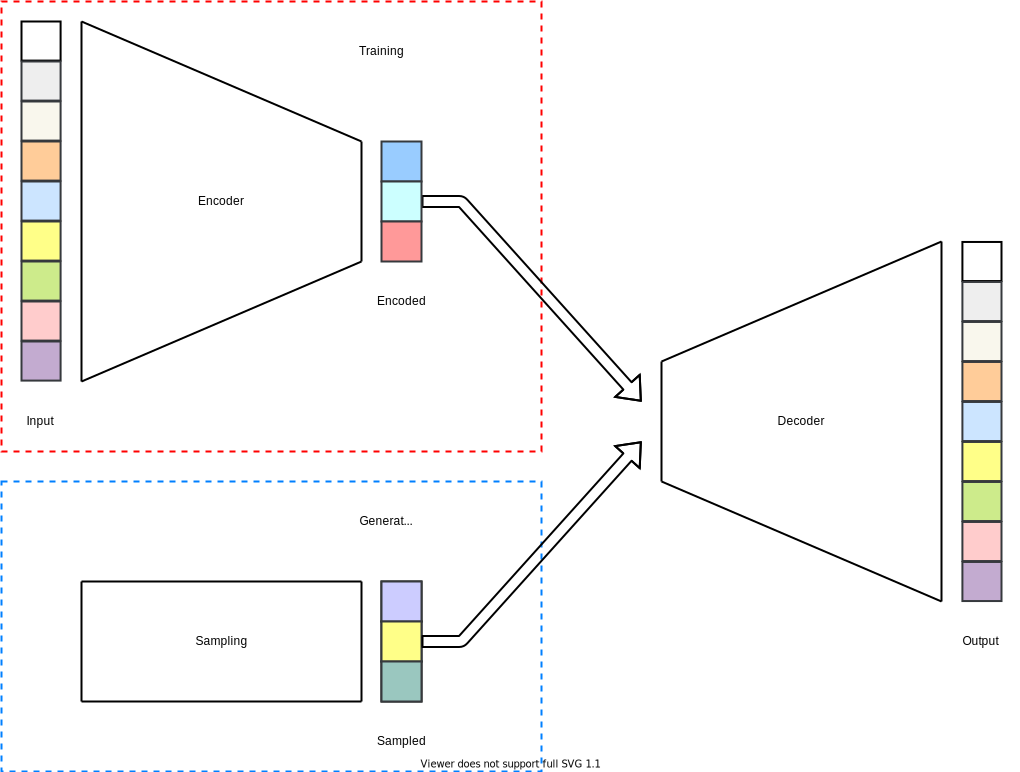
\includegraphics[width=\columnwidth]{figs/VAE_diagram.pdf}
    \caption{Overall VAE pipeline. One can generate new data by decoding points that are randomly sampled from the latent space. The quality and relevance of generated data depend on the regularity of the latent space.}
    \label{fig:vae}
\end{figure}

One way to attain these properties is to add a regularization term in the loss function.
In practice, this is done by enforcing distributions to be close to a standard normal distribution: covariance matrices are enforced to be close to the identity, preventing punctual distributions, and means to be close to 0,
prevent distributions from being too far apart from each other.

\subsection{Encoder and Decoder}
\textit{Encoders} and \textit{decoders} are neural networks. In the case of VAEs, the former takes an input $x$ and outputs the parameters of the probability distribution (assumed Gaussian with diagonal covariance) of its representation $z$ in the latent space. The latter takes the representation $z$ as an input and outputs an estimate $\hat{x}$ of the model's input $x$. However in the case of VQ-VAEs, due to their quantization properties, we can have the encoder directly outputs a vector in latent space.

The architecture of encoders and decoders will depend on the data at hand, but given that we are working with images, a convolution neural network seems to be the best choice. One of the architectures we developed thus alternates layers of convolution with downsampling (with use of a maxpool layer), a non-linear activation (ReLU) and Batch Normalization along the channel dimension. Finally, dense layers, also applied along the channel dimension, embed the convnet ouput into the latent space before quantization (see \autoref{fig:encoder_architecture}). The decoder follows this architecture in exact inverse order, replacing downsampling with upsampling and convolutions with transpose convolutions. Note that our implementation allows for a parametric instantiation of different shapes and numbers of layers, enabling quick testing. 

\begin{figure}
    \includegraphics[width=\columnwidth]{figs/encoder.pdf}
    \caption{Architecture of our Convnet Encoder. Dotted lines imply adding similar layers as needed, since the exact number and shape of layers is specified at instantiation.}
    \label{fig:encoder_architecture}
\end{figure}

While a VAE's prior and posterior distributions $p(z)$ and $q(z|x)$ are often Gaussian, the VQ-VAE is caracterized by the discretisation of its latent space, allowing a vector quantization inspired training~: the prior and posterior distributions are categorical, so that the latent representation $z_e$ of an input $x$ indexes an embedding table.

\subsection{Quantization Layer}

Figure~\ref{fig:VQVAE} highlights the Vector Quantization Layer, absent from traditionnal VAEs. This layer indexes values to an embedding space with an argmin~; this prevents backpropagation. Instead of flowing through the quantization layer, the gradient is copied from the layer's output to its input.
The quantization layer operates as follows~: a latent embedding space $e\in \RR^{K \times D}$ is introduced, where $K$ is the size of the discrete latent space, and $D$ is the dimensionality of each embedding vector $e_i$. The encoder network's output $z_e(x)$ is mapped to the nearest embedding vector $e_i$~:
\begin{equation}
    z_q(x)=e_k,\text{ where }k=\argmin_j\|z_e(x)-e_j\|_2,
\end{equation}

so that $z_q(x)$ is $z_e(x)$'s nearest embedding. This is the value that is passed to the decoder.

\subsection{Loss function}

The VQ-VAE's loss function has 3 components. The first one is the \textit{reconstruction loss}, optimizing both the encoder and the decoder, and is given by $\log p(x|z_q(x))$. As stated before, the gradient does not flow through the Vector Quantization layer~: the embedding step cannot be updated with the reconstruction loss. Vector Quantization is used for this purpose~: it makes use of the $l_2$ error between the encoded input $z_e$ and the embedding vectors $e_i$ in order to move the latter towards the former, as shown in the second term of \autoref{eq:vqvae_loss}. Finally, a third term, the \textit{commitment loss}, is added. It ensures that the embedding space is learnt at the same rate as the encoder parameters. Otherwise, the embedding space would grow arbitrarily as a result of it not training as fast as the encoder, implying a growth in the the output as well. 

\begin{equation}
\begin{split}
    L = & \log p(x|z_q(x)) + \|\sg[z_e(x)]-e\|_2^2\\
    & +\beta\|z_e(x)-\sg[e]\|_2^2
\end{split}
    \label{eq:vqvae_loss}
\end{equation}

In \autoref{eq:vqvae_loss}, $\sg$ states for the stop-gradient operator that is defined as identity at forward computation but whose gradient remain zero. In this way, the decoder optimizes the first term only, the encoder optimizes the first and third terms and the embedding vectors are optimized by the middle loss term.

\subsection{Discrete latent space}

Similar to traditional VAE, VQ-VAE can be used to generate new samples looking similar to the ones from the dataset by decoding artificial samples from the latent space. However, the latent space being a finite set of vectors, it is not ensured that it represents well the data. We therefore implemented three different techniques to enforce the embeddings to fit the data.

\paragraph*{Codebook initialization}

By initializing the codebook with random values, an issue can be that some embeddings would not have the same order of magnitude than the encoded data, which can lead to unused codes and very high gradients at the beginning of the training. In order to prevent such phenomenon, we initialize our codebook as a random subset of the first batch that the quantization layer receives during training. Assuming that this first batch is representative of the dataset, this simple technique enables to enforce the embeddings to be close to the data it is supposed to represent from the beginning of the training phase.

\paragraph*{Codebook random restarts}

Similar to traditional VAEs suffering from posterior collapse, VQ-VAEs are known to suffer from codebook collapse, wherein all encodings get mapped to a single or few embedding vectors while the other embedding vectors in the codebook are not used, reducing the information capacity of the bottleneck. To prevents this, we applied a technique proposed in \cite{Jukebox}, which consists in reinitializing embeddings which are not used enough by replacing their value by a random sample from the batch the quantization layer is training on. In fact, since each embedding receive gradients from the inputs of the quantization layer that are close to it, an embedding which is far from the training data will never be updated. These random restarts aim at overcome this issue by artificially preventing such situation. Similar to codebook initialization described above, they are therefore supposed to avoid part of the codebook from being unused, thus mitigating codebook collapse.

\paragraph*{Exponential Moving Averages}

Thanks to the $\sg$ operator in \autoref{eq:vqvae_loss}, the second term of the VQ-VAE loss is used only to update the codebook. An alternative to this solution that speeds up training is not to include this term in the loss but to update the codebook \emph{alla mano} instead, like for standard Vector Quantization techniques.

For an embedding $e_i$, let $\{z_{i,1}, z_{i,2}, \dots, z_{i,n_i}\}$ be the set of the $n_i$ outputs from the encoder whose closest embedding is $e_i$. The loss for the embedding $e_i$ is
\begin{equation}
    \sum_{j=1}^{n_i} \| z_{i,j} - e_i \|_2^2
\end{equation}
which has an optimal closed-form solution:
\begin{equation}
    \widehat{e}_i = \frac{1}{n_i} \sum_{j=1}^{n_i} z_{i,j}
\end{equation}

However, since the quantization layer receives batches instead of the whole training set at once, such updates could lead to numerical instability. Therefore, Exponential Moving Averages (EMA) updates are done instead for the embeddings to move smoothly:
\begin{equation}
    \begin{aligned}
       N_i^{(t)} &= \gamma N_i^{(t-1)} + (1 - \gamma) n_i^{(t)} \\
       m_i^{(t)} &= \gamma m_i^{(t-1)} + (1 - \gamma) \sum_j z_{i,j}^{(t)} \\
       e_i^{(t)} &= \frac{m_i^{(t)}}{N_i^{(t)}}
    \end{aligned}
\end{equation}
with $0 < \gamma < 1$. In practice, we chose $\gamma = 0.95$.

\section{The MNIST Dataset}\label{sec:MNIST}

\subsection{Presentation of the dataset}
The MNIST dataset is a subset of the larger NIST dataset. It includes grayscale images of handwritten numbers, in a train set of 60000 examples and a test set of 10000 examples. The images' low resolution ($28 \times 28$ px) leads to shorter computation times from the network, meaning that this dataset is particularly useful for verifying a model's behavior while implementing it. The implemented VQ-VAE is therefore trained with the MNIST dataset for some number of epochs, in order for it to be able to regenerate any picture in the set. 

\subsection{Reconstructing the input}

\begin{figure}[ht]
    \centering
    \includegraphics[width=\columnwidth]{figs/loss.pdf}
    \caption{Recorded loss of the training model}
    \label{fig:loss}
\end{figure}

For reconstructing images from the MNIST dataset, each 28 $\times$ 28 px input image is encoded to a 20 $\times$ 20 codemap of 16 discrete codewords. \autoref{fig:loss} shows that the loss function expectedly converges to a value around $10^{-2}$. The loss does not seem to decrease in a significant way beyond the fifth epoch. Equivalent or better results could probably be obtained with a shorter training by adjusting the encoder's content, which only performs two 2D convolutions in this example, as performance is not the focus here.
A small sample taken from the testing results obtained after 10 epochs is displayed on \autoref{fig:MNIST_test}~: it appears that the model has properly learnt how to recreate its input, and that the final loss computed while training ($\simeq$ 0.011) is low enough for the model's output to provide convincing reconstructions of the input images.

\begin{figure}[ht]
    \centering
    \includegraphics[width=\columnwidth]{figs/MNIST_test.png}
    \caption{Test input (left) and network output after 10 epochs (right)}
    \label{fig:MNIST_test}
\end{figure}

\section{The NSynth Dataset}\label{sec:NSynth}
\subsection{Presentation of the dataset}
NSynth is a dataset containing 306 043 audio files of individual musical notes, sampled at 16kHz from 1006 instruments from commercial sample libraries \cite{NSynth}. The sounds are generated for each instrument by ranging over every pitch of a standard MIDI piano (when the instrument is capable of it), for 5 distinct velocities. It permits our model to be trained on data that is closer to the final purpose of the project. 

Because of the size of the complete dataset, only its validation and test subsets are used for training and testing the model respectively, as it reduces the amount of time required to go through each epoch. A filtering function is also used, in order to train the model on samples coming from specific instruments for example. The data that is fed to the encoder must not be the direct audio files taken from the dataset, but their time-frequency representation.

\subsection{Time-frequency representation}
As explained in Section~\ref{sec:introduction}, this project involves computing the signal's spectrogram. It is based on the complex-valued Fourier Transform~: representing it on an image requires to make a choice regarding the way that magnitude and phase are used in the model.

The approach here is to only train the model on the magnitude of the spectrogram as it conveys all the information that our model has to learn, i.e. the sound magnitude of musical notes relative to time and frequency. For reconstructing audio data, several methods can be used. The phase of the original signal can be carried over to the output of the VQ-VAE, or it can be discarded and favored by a phase-reconstruction method such as the Griffin-Lim algorithm, based on redundancies of the spectrogram.

Another existing method is to represent magnitude with brightness and the derivative of the phase with color. It allows the model to learn the behavior of every parameter of the sound instead of relying on other data or on an algorithm~\cite{NSynth}. 

\subsection{Reconstructing the input}
The reconstruction of the input images is attempted in the same way as described for the MNIST dataset, with a codemap of a different shape and more codewords. However, the change in scale of the input appears to have made apparent a problem in the model that prevent it from learning correctly, despite our numerous experiments with various hyperparameters (learning rate, codebook size, latent dimension, number of convolutions, etc.) \autoref{fig:reconstruction} shows the best-looking reconstructed spectrograms we get with one of our models.

\begin{figure*}
    \centering
    \includegraphics[width=0.48\textwidth]{figs/zot1.png}
    \includegraphics[width=0.48\textwidth]{figs/zov1.png}
    \includegraphics[width=0.48\textwidth]{figs/zrt1.png}
    \includegraphics[width=0.48\textwidth]{figs/zrv1.png}
    \caption{Examples of spectrograms reconstructed by our model on training data (left) and validation data (right). The originals are to the top and the reconstructions down below. Even if the overall shape of the original spectrogramm is sometimes visible in the reconstructions, these results are not as accurate as the ones we reach on MNIST.}
    \label{fig:reconstruction}
\end{figure*}

\section{Experiments/Results}\label{sec:experiments}

Because of the model's trouble reconstructing large inputs such as spectrograms, this section exclusively focuses on applying inpainting to the MNIST dataset.

By applying transformations on the codemap encoding of a spectrogram we can create different type of audio effects on the decoded signal. One way to create effects is by applying simple transformations on the whole codemap, for example by adding noise or remove values. Another way would be to resample some elements of the codemap encoding with inpainting methods in order to modify some features of the sound.

\subsection{Simple transformations on codemaps}

A simple transformation possible on a codemap encoding of an image is to remove channels in order to obtain a lower resolution image. The \autoref{fig:MNIST_Transform0} display the transformation of a MNIST image by keeping only one channel on the codemap encoding of the image.

\begin{figure}[ht]
    \centering
    \includegraphics[width=0.4\columnwidth]{experiments/MNIST_transformations/0_orig.PNG}
    \includegraphics[width=0.4\columnwidth]{experiments/MNIST_transformations/0_low.PNG}
    \caption{MNIST image (left) and the image decoded after removing all but one channel in the codemap encoding of this image (right)}
    \label{fig:MNIST_Transform0}
\end{figure}

We also experiment mixing the codemap values between images before decoding them. The \autoref{fig:MNIST_Transform1} present an example of one of this experiments, the results are really close to a mix between the original images.

\begin{figure}[ht]
    \centering
    \includegraphics[width=0.8\columnwidth]{experiments/MNIST_transformations/1_orig.PNG}
    \includegraphics[width=0.4\columnwidth]{experiments/MNIST_transformations/1_mix.PNG}
    \caption{Two MNIST images (top) and the image decoded after mixing the codemaps of both these images (bottom)}
    \label{fig:MNIST_Transform1}
\end{figure}

\subsection{Codemap Inpainting}

The inpainting process allow to modify an image in order to restore part of it or to add/remove elements of the image. There is a lot of different digital inpainting methods, going from simple probabilistic model to deep learning neural model. Codemaps can be seen as really low-resolution images so we don't need complex inpainting method. A simple and effective inpainting process for our model is the Bayesian approach.

The idea behind the naives bayes classifier is to create a simple class distribution from the list of neighbouring points and their associated classes. With this distribution we can have an estimation for the class of any other point in the plane. In the case of codemap inpainting, the points are the elements of the codemap and the classes are the values of these points.

\begin{figure}
    \includegraphics[width=\columnwidth]{figs/inpainting.pdf}
    \caption{Overall VQ-VAE training and inpainting pipeline. The Encoder, Decoder, and Quantizer are first trained on data, then when parts of the input data are removed, we can apply a Naive Bayes Classifier to reconstruct a likely codemap in discrete latent space. Applying the decoder allows to return to an "inpainted" image.}
    \label{fig:inpainting}
\end{figure}

Considering a codemap encoding of a spectrogram, we can do inpainting with the Bayesian approach by the following process:
\begin{enumerate}
    \item Select an element of the codemap.
    \item Get a list of a certain number of neighbors of this point and the values associated (we can choose the elements that are only along the frequency axis or the time axis or both).
    \item Create a gaussian naive bayesian distribution with as training samples the list of neighbors, and as target values (classes) the values of this points.
    \item Use the distribution created to predict and replace the value of the originally selected element.
\end{enumerate}
We repeat this process for every element of the codemap we want to resample. This method can also be made autoregressive to keep consistency with the values predicted by the bayes classifier.

The \autoref{fig:MNIST_inpainting} present two examples of autoregressive inpainting on a small area of an image from the MNIST dataset. As expected the bayesian classification is really sensitive to the points closest to the elements to sample and the values resampled are mostly either equal to the minimum value or the maximum value of the image.

\begin{figure}[ht]
    \centering
    \includegraphics[width=0.4\columnwidth]{experiments/MNIST_inpainting/0_0_box.PNG}
    \includegraphics[width=0.4\columnwidth]{experiments/MNIST_inpainting/0_0_res.PNG}
    \includegraphics[width=0.4\columnwidth]{experiments/MNIST_inpainting/0_1_box.PNG}
    \includegraphics[width=0.4\columnwidth]{experiments/MNIST_inpainting/0_1_res.PNG}
    \caption{MNIST image with the area to resample in blue (left) and the image obtained after inpainting with naive bayes classification (right)}
    \label{fig:MNIST_inpainting}
\end{figure}

\section{Energy considerations}\label{sec:energy}

Learning lightweight representations of audio effects is necessary for real-time applications (e.g. interactive composition) or for deployment on devices with limited computational power such as mobile phones or embedded systems.
Moreover, this approach takes a stand against the common approach of deep learning research which consists in training ever-larger models on a huge amount of data, thus inducing increasingly higher environmental costs.

\paragraph*{Methodology}

In order to estimate the overall energy consumption of our experiments, we followed a simplified version of the methodology introduced in \cite{Energy}. In this paper, the total power consumption of the training is estimated as the sum of the one of the CPU, GPU and DRAM draw, multiplied by the so-called Power Usage Effectiveness (PUE) coefficient, which is about 1.58. Then the induced CO$_2$ emissions are assumed to be proportional to the total energy consumption, with a multiplying coefficient of 0.477.

In our project, we assume that the power of the CPU and DRAM draw is marginal compared to the one of the GPU, which implies that the total power consumption is proportional to the GPU power. Since we realized all our experiments on a single GPU, it follows that the estimated CO$_2$ emissions of a training of duration $T$ are:
\begin{equation}
    \text{CO}_2\text{e} = 0.477 \times 1.58 \int_0^T p_{\text{GPU}}(t) \ \text{d}t
    \label{eq:co2}
\end{equation}
where $p_{\text{GPU}}(t)$ denotes the power of the GPU at time $t$. In practice, $p_{\text{GPU}}$ remains almost constant during the training, leading to a linear correlation between its CO$_2$ emissions and its duration (see \autoref{fig:co2}).

In practice, exists more precise tools for estimating deep learning CO$_2$ emissions such as \emph{carbontracker}, which logs CO$_2$ consumption during training as our own tracker, but also aims at predicting the total carbon footprint of the training~\cite{Carbontracker}. Moreover, contrary to our model, it takes into account many parameters (e.g. GPUs model, country where the training is performed, etc.) to provide more accurate estimations than the ones computed with \autoref{eq:co2}.

\paragraph*{Experiments}

\begin{figure}
    \centering
    \includegraphics[width=0.49\textwidth]{figs/co2.pdf}
    \caption{Instantaneous GPU power (top) and estimated CO$_2$ emissions (bottom) over time induced by training the model on the NSynth dataset, for different grid sizes. All models have about 66 K trainable parameters.}
    \label{fig:co2}
\end{figure}

We implemented a CO$_2$ tracker to record and measure the energy consumption of our experiments over time. This tracker acts almost like a Linky meter: it measures the power of the GPU at the end of each epoch, then estimates the induced CO$_2$ emissions using \autoref{eq:co2} and finally logs the results on TensorBoard, thus enabling to track the consumption of energy in real-time while training as any other metric.

From our different experiments, it appears that changing the values of the hyperparameters of the program (number of codewords, dimension of the latent space, etc.) has no significant influence on the energy consumption. The only parameter that seems to have an influence is the downsampling rate of the encoder, i.e. the difference between the spectrogram original size and the latent grid sizes. In particular, it is worth noticing that the architecture used for the encoder/decoder and the number of trainable parameters seems not to have any influence on the energy consumption. In an ecological point of view, learning small but powerful representations for audio effects seems therefore to be the best option. However, we only trained relatively small models (up to six convolutional layers) on a small dataset, so we cannot ensure that our conclusions are still relevant for "real-scale" deep learning models.

\section{Conclusion and future work}\label{sec:conclusion}

\subsection{Achieved work}

This document presents how VQ-VAEs can be used to produce lightweight interactive effects~: their discrete latent space allows for a very compact and compressed representation of the input signal, that can be easily modified in order to produce interesting and creative transformations of the input. To that end, selected parts of the input image's codemap are replaced by an estimation based on a gaussian naive Bayesian distribution. We produced a modular implementation of VQ-VAE that fully supports smart codebook initialization, codebook random restarts and Exponential Moving Averages updates. We also realized several experiments on MNIST to illustrate this application of VQ-VAEs, and also tried to apply it to NSynth but unfortunately without success.

The environmental cost induced by training a model is also taken into account, as it represents an important subject matter for which raising awareness is essential. The VQ-VAE's CO$_2$ consumption is measured for several downsampling rates, exhibiting the appeal of lightweight models, particularly for devices with limited computational power.

\subsection{Perspectives}

Despite of our promising results on MNIST, this work can be completed and expanded upon in several ways~:

\paragraph*{Overall model} First, the model seems to have problems or bugs that prevent it from learning properly on large images such as spectrograms. These have to be addressed in order for the model to be used in a musical context.

\paragraph*{Data loading} For this project, we only used relatively small neural networks and therefore considered it would be sufficient to train our networks only on the validation set of NSynth. Moreover, since we did not even use a big dataset, we did not perform any data augmentation. Finally, the input of our model is a spectrogram magnitude, which is quite common for that use case, but might not be the most efficient representation. Using the phase or its derivative as a channel may give extra information to the neural network and thus improve our results, as in~\cite{PhaseFeatures}. Another relevant option could be to use mel-spectrograms~\cite{MelSpectrogram} instead of traditional ones.

\paragraph*{Architecture} The architecture of both the encoder and decoder can be refined, as they have been kept rather simple throughout the project. Adding residual skip-connexions has been shown to be relevant for various tasks in deep learning and could therefore be useful in our case~\cite{Resnet}. Moreover, even if treating spectrograms as images is convenient since it enables to use MNIST as a toy dataset, replacing convolutions by an architecture that is designed to work better on music, such as Wavenet-style autoencoders~\cite{Wavenet,NSynth}, could lead to better results. Combining codemaps of different resolutions, as suggested in \cite{VQVAE2}, could also improve our results.

\paragraph*{Inpainting} Using naive Bayes classification for inpainting seems to provide promising results but using deep neural networks architectures could definitely lead to better results. Transformers~\cite{Transformers} is nowadays the most common architecture for sequence deep models, but they suffer from one major drawback: these are slow models that need a huge amount of computational power, thus not being really adapted to our purpose since we aim at providing a model that can infer almost in real-time and that has a low energy consumption. However, exists some improvements to the traditional Transformer architecture that precisely overcome these drawbacks, e.g. Linear Transformers~\cite{LinearTransformers}. Using such architecture could be a proper way to increase the quality of our inpainted spectrograms for little extra energy consumption (at least less than with traditional Transformers).

\paragraph*{Energy consumption}

As explained in \autoref{sec:energy}, our methodology for estimating the energy consumption of our models leads to rough estimations and could be improved. Moreover, since the GPU power seems to be almost constant over time, we only measured it at the end of each epoch, which might be inaccurate. Using a multithreaded CO$_2$ tracker which records the GPU power every second instead of at the end of each epoch would probably provide better estimations, but we found implementing such a tracker out of the scope of this project. For real-case applications, using trackers such as the one described in \cite{Carbontracker} may be a relevant option.

% For bibtex users:
\bibliography{ML-project}

% For non bibtex users:
%\begin{thebibliography}{citations}
%
%\bibitem {Author:00}
%E. Author.
%``The Title of the Conference Paper,''
%{\it Proceedings of the International Symposium
%on Music Information Retrieval}, pp.~000--111, 2000.
%
%\bibitem{Someone:10}
%A. Someone, B. Someone, and C. Someone.
%``The Title of the Journal Paper,''
%{\it Journal of New Music Research},
%Vol.~A, No.~B, pp.~111--222, 2010.
%
%\bibitem{Someone:04} X. Someone and Y. Someone. {\it Title of the Book},
%    Editorial Acme, Porto, 2012.
%
%\end{thebibliography}

\end{document}

